% Базовый проект
% Реализация инструментальных средств преобразования онтологических описаний в структуры UML с последующей их интерпретаций в виде программного кода компонент ИС и АРМ.

% РФФИ

% Разработка специализированной системы трансформации платформонезависимой модели, ориентированной на поддержку современных средств разработки интернет-приложений, функционирующих в среде Linked Open Data.

\documentclass[12pt]{article}
\RequirePackage[a4]{}
\RequirePackage{luatextra}
\RequirePackage[a4paper,margin=2cm,includeheadfoot,nofoot]{geometry}
% \RequirePackage[a4paper,margin=2cm,includeheadfoot,nofoot,showframe]{geometry}
\RequirePackage{polyglossia}
\RequirePackage{indentfirst}
\RequirePackage{doi}
\RequirePackage[protrusion=false,expansion=false]{microtype}
\SetProtrusion
    [name=std]
    {
      encoding={utf8},
      family=*}
    {
    « = {300,     },
    » = {    , 300},
    „ = {300,     },
    “ = {    , 300},
    ( = {300,     },
    ) = {    , 300},
    ! = {    , 300},
    ? = {    , 300},
    : = {    , 300},
    ; = {    , 300},
    . = {    , 300},
    - = {    , 300},
   {,}= {    , 300}
    }
%\DeclareMicrotypeSet{t2atext}{}
%\UseMicrotypeSet{t2atext}
\microtypesetup{protrusion=true,expansion=true}
\newfontfeature{Microtype}{protrusion=default;expansion=default;}

\setmainlanguage{russian}
\setotherlanguage{english}
\setkeys{russian}{babelshorthands=true}
\usepackage{minted}
\usemintedstyle{bw}
\setminted{fontsize=\small}
\usepackage{hyperref}
\hypersetup{
    % bookmarks=true,         % show bookmarks bar?
    unicode=true,          % non-Latin characters in Acrobat’s bookmarks
    pdftoolbar=true,        % show Acrobat’s toolbar?
    pdfmenubar=true,        % show Acrobat’s menu?
    pdffitwindow=false,     % window fit to page when opened
    pdfstartview={FitH},    % fits the width of the page to the window
    %pdftitle={},    % title
    %pdfauthor={Author},     % author
    %pdfsubject={Subject},   % subject of the document
    %pdfcreator={Creator},   % creator of the document
    %pdfproducer={Producer}, % producer of the document
    %pdfkeywords={keyword1, key2, key3}, % list of keywords
    %pdfnewwindow=true,      % links in new PDF window
    colorlinks=true,       % false: boxed links; true: colored links
    linkcolor=black,          % color of internal links (change box color with linkbordercolor)
    citecolor=black,        % color of links to bibliography
    filecolor=black,      % color of file links
    urlcolor=black,           % color of external links
    final=true
  }

\defaultfontfeatures{Ligatures=TeX}
\setmainfont{Times New Roman}
\setromanfont{Times New Roman}
\setsansfont{Arial}
\setmonofont{Courier New}


\newfontfamily{\cyrillicfont}{Times New Roman}
\newfontfamily{\cyrillicfontrm}{Times New Roman}
\newfontfamily{\cyrillicfonttt}{Courier New}
\newfontfamily{\cyrillicfontsf}{Arial}


\addto\captionsrussian{%
  \renewcommand{\figurename}{Рис.}%
  \renewcommand{\tablename}{Табл.}%
}
\setlength{\parindent}{1cm}

% Поля страницы: верхнее, нижнее, левое, правое – 2 см.

\setmainfont{Times New Roman}
\tolerance=1
\emergencystretch=\maxdimen
\hyphenpenalty=10000
\hbadness=10000
\pagestyle{empty}
\begin{document}
%УДК 004.4'244

\title{Инструментарий анализа, классификации и интерпретации
сцен}

\maketitle

\begin{abstract}
  Рассматриваются современные средства реализации этапов анализа,
  классификации и интерпретации сцен, которыми, в частности, выступают
  тексты и модели их интерпретации, полученные в результаты применения
  средств машинного обучения. Средства базируются на использовании
  стандартизованных моделей представления данных и технологий логического
  вывода, позволяющие в высокой степени независимо от других средств
  разрабатывать процедуры анализа сцен. Процедура анализа представляет
  собой реализацию сценария, характеризующего сцену. Соотнесение некоторой
  сцены сценарию порождает заключение о конкретном классе сцены в
  некоторой системе классификации вместе с дополнительными параметрами,
  характеризующими сцену. Интерпретация сцены или набора сцен представляет
  собой трансформацию распознанных классификаций в модели другого вида.
  Приводится пример реализации технологии, используемой в синтезировании
  программного кода программной системы по набору абстрактных моделей,
  реализованных в языке Logtalk.
\end{abstract}

\section*{Введение}

Термин \emph{искусственный интеллект} (ИИ) в настояще время чаще всего
связывают с моделями, основанными на машинном обучении, в том числе,
нейронными сетями, включающими алгоритмические структуры свертки,
генерирующими нейронными сетями, моделями регрессии, таксономии,
классификации на основе машинного обучения и т.п. Известным ограничением
применимости подходов к решению задач ИИ, основанных на машинном
обучении (МО), являются невозможность интерпретации получаемых моделей в
виде процедуры трансформации данных: нейронная сеть -- это набор
коэффициентов, моделирующих синапсы и подобные им структуры соединений
между элементами (нейронами). Другим важным ограничением МО является
сложность построение моделей МО, распознающих свойства систем, состояние
которых меняется во времени (\emph{динамических систем}). Например,
предобученные модели МО применяются для анализа и распознавания объектов
на растровых изображениях (лиц людей, движущихся объектов), но весьма
сложно строить системы принимающие решения о наличии или отсутствии
тенденции объектов на изображении входить в свое города коллизию.
Например, на видеоизображении могут быть две группы людей, которые стоят
лицом друг к другу. Аналогично и с текстами: последовательность
сообщений между участниками общения могут формировать некоторый план
саботажа промышленного объекта.

Задача распознавания возможных намерений и действий участников сцены
реализуется анализом динамики взаимодействия субъектов общения -- каким
образом объекты переходят из состояния в состояние, какие свойства
меняются при каждом переходе, каков допустимый набор этих состояний,
какие состояния обладают критическими признаками для принятия решения. В
результате надо принять решение о том, соответствует ли сцена
необходимому набору признаков.

Решение этой задачи основывается на построении иерархической системы
моделей, где на нижнем уровне располагаются результаты распознания и
классификации объектов (индивидуальных фраз в текстовых сообщениях,
тональностей в аудиосообщениях, кадров изображений) методами МО, выше
представлены модели статического аспекта сцен на кадрах, выраженных в
свойствах объектов и связей между ними. Уровни выше описывают
информационный поток сообщений как набор сцен, который, в свою очередь
также является сценой. Сопоставление конкретной распознанной сцены
одному из заданных сценариев есть решение задачи классификации. При этом
в качестве результата получаем не только решение о классе, но и
параметры элементов сценария.

Интерпретация сценария зависит от поставленной задачи (целевого
сценария). Сама распознанная сцена и ее соответствие сценарию
представляет собой модель интерпретации высокого
уровня. Для реализации других вариантов интерпретации сцен, а также
реализации процедур синтеза информационных объектов, необходимо задания
контекстной модели. Система искусственного интеллекта (ИИ), основанная
на формализованных знаниях, при помощи анализа результата распознавания
и модели контекста порождает соответствующий вариант интерпретации или
целевой объект.

В статье рассмотрен вариант реализации данного подхода, обеспечивающий
синтез программного кода \emph{dataflow}-модулей, элементов интерфейса
пользователя, декларативных структур и т.п. для программной системы
Rapidminer studio (RS) на основе анализа программного кода модулей в
пакете Mothur. Процедура распознавания на нижнем уровне анализирует
исходный код, используя регулярные выражения. Далее результаты
объединяются в модели структур данных, относимых к разным классам.
Следующий уровень уже представляет описание модулей пакета Mothur, затем
получается модель всего пакета.

Целью интерпретации -- является синтез модулей RS, позволяющих
пользователю представлять вычислительный процесс как последовательность
модулей Mothur в графовой структуре потока исполнения. Модель контекста
представляет собой формализованную процедуру творческой деятельности
программиста, реализующего программный код по спецификации --
распознанной структуре пакета Mothur -- и в соответствии с требованиями
интерфейса прикладного программирования (API) встроенных модулей RS.

Этапы анализа исходного кода реализуются на Python (уровень регулярных
выражений), Prolog/Logtalk \cite{logtalk} -- остальные уровни анализа, классификации и
интерпретации. Исходные данные -- репозиторий исходного кода C++ Mothur,
базовые характеристики и связи между ними представляются в виде графов
знаний на основе технологий семантического веба. Объекты верхнего уровня
-- объекты Logtalk, связывающие элементы (тройки) графа друг с другом
семантическими отношениями более высокого абстрактного уровня. Модель
контекста представляется набором взаимодействующих друг с другом
объектов (компонент) Logtalk.

\section{Распознавание структуры прикладного пакета}

Прикладной пакет Mothur используется для анализа данных высокопроизводительного секвенирования РНК оборудованием фирмы Illumina MiSeq.  Процесс анализа заключается в последовательном запуске модулей пакета (более 140 штук), экспорта/импорта данных в сторонние пакеты (Usearch, QIIME2), подготовки диаграмм, визуализирующих результаты (R, Excel).  Данный процесс называется \href{https://mothur.org/wiki/miseq_sop/}{MiSeq SOP} (MiSeq Standard operating procedure), сценарий.  По своей сути каждое исследование представляет собой реализацию варианта сценария MiSeq SOP.

Для проведения анализа исследователь программирует сценарий, сообщая входные данные (набор файлов).  Результаты исполнения модулей также помещаются в файлы, которые идут на вход в другие модули.  Кроме входа и выхода в модуле задаются управляющие параметры.  Представленная схема соответствует вычислительной парадигме \emph{dataflow} \cite{dataflow}, а программный комплекс Rapidminer studio (RS) позволяет такие схемы представлять визуально.  Идеей проекта \cite{zont19} выступало создание библиотеки RS для представления MiSeq SOP, что призвано дать возможность биологам самостоятельно проводить анализ данных высокопроизводительного секвенирования нового поколения.

\subsection{Представление данных}
% Здесь надо сказать о том, что для ЛООП удобен формат RDF, даже в сранении с XML.

Исходными данными для автоматического порождения модулей RS является исходный код Mothur, представленный на языке программирования C++.  Исходный код анализировался при помощи регулярных выражений, процедура анализа реализована средствами библиотек Python.  В результате формируется \emph{граф знаний} \cite{kg} о спецификации прикладного пакета.

Граф знаний (ГЗ) -- это множество троек вида \texttt{<субъект, предикат, объект>}.  Тройки задают отношение \texttt{предикат(субъект, объект)} в нотации языка Prolog.  В настоящее время инструментальные средства ГЗ активно развиваются: создаются системы хранения и доступа к данным и знаниям ГЗ, формируются стандартизованные модели представления предметных областей, разрабатываются методики совместного использования этих моделей для описания информации в конкретных прикладных задачах.  Основная цель этих исследований состоит в создании среды интегрирования информации в распределенных подсистемах, включающих решение задач распознавания.

Приведем пример представления исходных данных описания модулей в прикладном пакете.
\begin{minted}[fontsize=\normalsize]{turtle}
@prefix xml: <http://www.w3.org/XML/1998/namespace> .
@prefix xsd: <http://www.w3.org/2001/XMLSchema#> .
ngsp:spec a ngsp:Specification ;  # Список модулей Mothur
    ngsp:module mothur:NoCommand,
        mothur:align-check,       # Align Check
        mothur:align-seqs,        # Align Seqs
# . . . . . # Команда Align Check
mothur:align-check a ngsp:Module ;
    ngsp:outputPattern [ a cnt:Chars ; # Способ формирования
            ngsp:parameterName "type" ;# имени выходного
            ngsp:pattern [ ngsp:patternString # файла
                    "[filename],align.check" ;
                    dc:identifier "aligncheck" ] ;
            cnt:chars # . . . .
# . . . . . # Описание свойств параметров модуля
mothur:align-check-idir-parameter a ngsp:Parameter ;
    ngsp:important false ;
    ngsp:multipleSelectionAllowed false ;
    ngsp:optionsDefault "" ;
    ngsp:required false ;
    ngsp:type mothur:String ;
    dc:title "inputdir" .

mothur:align-check-map-parameter a ngsp:Parameter ;
    ngsp:important true ;
    ngsp:multipleSelectionAllowed false ;
    ngsp:optionsDefault "" ;
    ngsp:required true ;
    ngsp:type mothur:InputTypes ;
    dc:title "map" .

mothur:align-check-name-parameter a ngsp:Parameter ;
    ngsp:chooseOnlyOneGroup "namecount" ;
    ngsp:important false ;
    ngsp:multipleSelectionAllowed false ;
# . . . . .
\end{minted}

Сценарии анализа задаются в виде методов объектов объектно"=ориентированного языка Logtalk, основанного на Prolog и позволяющего использовать средства объектно"=ориентированного программирования для манипуляции набором знаний Prolog"=а. Эффективный доступ к тройкам обеспечивается при помощи низкоуровневого слоя библиотеки SWI-Prolog \texttt{rdflib}, реализованного на языке C.  Объекты"=элементы сценария представляется в виде экземпляров Logtalk, хранящих состояние (stateful objects).

\begin{minted}{logtalk}
:- object(query(_XMI_)).
  :- public([class/2, attribute/3, method/3]).
  class(Name, ID):-                            % Распознавание
  _XMI_::rdf(ID,rdf:type,uml:'Class'),       % класса
  _XMI_::rdf(ID,rdfs:label, literal(Name)).

  attribute(Name, ClassID, ID):-               % ...атрибута...
  _XMI_::rdf(ClassID, xmi:ownedAttribute, ID),
  _XMI_::rdf(ID, rdfs:label, literal(Name)).

  method(Name, ClassID, ID):-                  % ...метода...
  _XMI_::rdf(ClassID, xmi:ownedOperation, ID),
  _XMI_::rdf(ID, rdfs:label, literal(Name)).
  % . . . . . . . . . . .
:- end_object.
\end{minted}

Модели могут ссылаться на внешние объекты, хранимые в других ГЗ, таких как, \texttt{DBPedia} и \texttt{Wordnet}.  Это, в свою очередь, позволяет среди разных процедур распознавания идентифицировать однозначно конкретные объекты.  Кроме того, из \texttt{DBPedia} можно получить локализованные названия ресурса, переводы терминов на другой язык.  Объекты Logtalk получают данные с этих ресурсов при помощи SPARQL-запросов.  Результаты распознавания представляются совокупностью объектов, которую при необходимости можно также сохранить в новый ГЗ, и, затем, применить к нему внешние алгоритмы, решающие специальные задачи.

По сути, сценарии -- это иерархические древовидные структуры, где каждый уровень отражает определенный уровень абстракции процесса распознавания.  Над объектами и сценариями нижнего уровня выполняется процедура анализа верхнего уровня по аналогии.  В конечном счете полученная иерархия объектов и сценариев подвергается интерпретации в виде трансформации в другие модели.  В данной задаче интерпретация структуры прикладного пакета представляет собой двухуровневую структуру. Верхний уровень -- это абстрактная структура модуля, представимая в абстрактном объектно-ориентированном языке, а нижний уровень соответствует исходному Java-коду модулей RS.

Язык Пролог с его ООП надстройкой оказался мощным инструментом для представления трансформаций.  Благодаря его простой декларативной структуре и возможности реализовывать различные интерпретации этих структур, он позволяет представлять все аспекты трансформации, начиная с импорта и хранения в оперативной памяти исходных моделей, распознавания и синтеза структур, до порождения текстов исходного кода.  И, в отличие от стандартных подходов, базирующихся на использовании специальных языков трансформации таких, как ATL, QVT и их аналогов \cite{azis,QVT,nikita}, Prolog позволяет не только выполнять трансформации, но и выходить за их рамки: использовать внешние программные библиотеки, не имеющие прямого отношения непосредственно к анализу и трансформации.  Logtalk выводит все на новый уровень, позволяя при помощи 1) инкапсуляции создавать фасадные объекты к исходным данным, выполняющие функции адаптеров, скрывающих сложные алгоритмы за их спецификациями в интерфейсе; 2) наследования манипулировать наборами правил баз знаний; 3) композиции реализовывать типичные сценарии решения задач в листовых вершинах, 4) перехвата сообщений фильтровать распознанные объекты в зависимости от контекста трансформации.

К такому достаточно универсальному варианту представления мы пришли в результате исследований различных подходов к заданию сценариев и правил трансформации, комбинируя различные языки программирования.  Интересным решением был вариант \cite{b2}, где правила представлялись комбинацией распознавателя, реализованного в виде пролог-предиката, а процедура трансформации реализовалась на языке Python как тело соответствующего метода.  Параметры метода предавались в параметры предиката.  Тело метода запускалось заново для каждого ответа распознающего предиката.  Сценарии реализовались в виде списков объектов и методов, последовательный запуск которых реализовывал синтез исходного кода объектов.  Для манипулирования наборами правил использовалась композиция на основе подмешивания (mixin) классов, не имеющих своего состояния.  Такой механизм реализовывал подход на основе типовых конфигураций (pattern-directed programming).

\subsection{Программирование трансформации}
% По рисунку из статьи ICIS'18.

Ограничения объема доклада позволяют разобрать только один пример представления процедуры трансформации верхнего уровня, не учитывающий какую"=либо специфику платформы и приемов программирования.
\begin{minted}{logtalk}
% ?- tr_package(sample,lp,cp)::tr(class,person,ID). % Тест
:- object(tr_package(_Package_, _Local_, _Global_)).
  tr(class, Class, ClassID):-   % Метод - трансформатор класса
    query(_Package_)::class(Name, ClassID),   % Распознавание класса
    ::new(Class, [instantiates(class)]),      % создание экземпляров -
    ::new(Attributes,[instantiates(attributes)]), % списков элементов
    ::new(Methods, [instantiates(methods)]), % класса
    Class::name(Name),          % Установить название класса.
    forall(::tr(attribute, Attribute, ClassID, _), % Трансформировать
        Attributes::append(Attribute)),            % его атрибуты
    forall(::tr(method, Method, ClassID,_),        % и методы
        Methods::append(Method)),
    Class::attributes(Attributes),    % Установить структурные
    Class::methods(Methods).          % элементы класса
:- end_object.
\end{minted}

Здесь \texttt{tr\_package/3} -- параметризованный объект, задающий шаг сценария трансформации \texttt{tr/\_}.  Объекты Logtalk (классы, экземпляры, протоколы, категории) -- это символы, находящиеся друг с другом в определенных отношениях.  При помощи параметров объектов можно задавать контекст для его методов.  В объекте \texttt{tr\_package/3} контекст задается тремя моделями \texttt{\_Package\_} -- PIM программной системы, \texttt{\_Local\_} -- перечень типов данных проекта (локальная библиотека), \texttt{\_Global\_} -- набор стандартных типов данных.  Эти три параметра задаются на уровне абстрактных сценариев согласно спецификации UML-2.4 \cite{GT}.  Параметризованный объект \texttt{query/1} получает в качестве параметра граф, где хранятся тройки и где следует распознавать структуры модели.  Объекты с параметрами позволяют обходиться без создания отдельных экземпляров класса, но при этом учитывать контекст в реализации методов.  Языковая структура \texttt{obj::method} -- это посылка сообщения (в терминологии Smalltalk) объекту \texttt{obj} или самому себе \texttt{::method}.  В объекте \texttt{query/1} реализован метод распознавания класса как структуры типа \texttt{uml:Class} с внутренними UML-идентификатором \texttt{ID} и именем (названием) \texttt{Name}.  Методы класса \texttt{::new/2} используются для создания экземпляров классов \texttt{class}, \texttt{attributes} и \texttt{methods}, которые, соответственно, помещаются в переменные \texttt{Class}, \texttt{Attributes}, \texttt{Methods}.  Для всех структур, представляющих сценарии нижнего уровня, заданы процедуры перевода в исходный код.

В результате генерируются следующие элементы проекта расширения RS для Mothur.
\begin{enumerate}
\item Исходные коды модулей Java для операций, включая базовые исполнительные механизмы, в частности запуск на выполнение модуля с передачей ему параметров;
\item Описание модулей в интерфейсе редактора RS в формате XML;
\item Описание иерархической структуры элемента управления для выбора модуля в процессе добавление в диаграмму.
\end{enumerate}
Таким образом, процедура трансформации реализует интерпретацию исходного кода Mothur в виде исходного кода модулей RS, и, в конечном счете в виде набора изображений"=блоков datafalow для пользователя"=предметника.  На рисунке~\ref{fig:ex} продемонстрирован пример использования полученного инструментария.  Зеленые блоки --  это блоки, сгенерированные при помощи разработанного инструментария, бежевые -- стандартные операции RS.

\begin{figure}
  \centering
   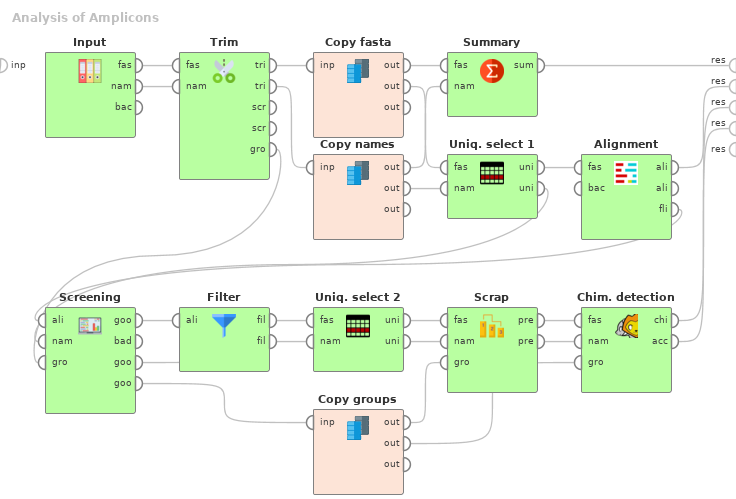
\includegraphics[width=0.8\linewidth]{Dataflow-color-en.png}
  \caption{Пример построения начальной фазы исследования согласно методике MiSeq SOP}
  \label{fig:ex}
\end{figure}

\section*{Заключение}

В работе представлен подход к синтезу программного кода подсистем
инструментального средства Rapidminer studio по исходному коду компонент
прикладного пакета Mothur (анализ данных высокопроизводительного
секвенирования РНК). Продемонстрированы средства реализации некоторых этапов
анализа, классификации и интерпретации исходного кода Mothur, в
результате приводящих к синтезу пакета Java, реализующего декларативную
часть модулей dataflow в Rapidminer studio. Внимание уделено вопросам
стандартизации представления и реализации этапов распознавания, решение
которых направлено на создание инструментальной среды разработки средств
анализа и интерпретации, где разные этапы в достаточной степени
независимы друг от друга.

Предложенный подход совершенствует существующие методы анализа текстов, основанные на синтаксическом и семантическом анализе, в направлении использования объектного логического языка для представления процедур анализа и трансформации, технологий Семантического веба (СВ) для представления предметной области в виде графов знаний и идентификации объектов.  Подходы, основывающиеся на СВ, позволяют эффективно производить интеграцию программных систем и реализовывать совместное многоагентное решение задач.  Обобщение представленного подхода позволит решать задачи, представляющие
интерес в системах автоматизации деятельности органов военного управления.

\textit{Исследование проведено в рамках проекта <<Методы и технологии облачной сервис-ориентированной цифровой платформы сбора, хранения и обработки больших объёмов разноформатных междисциплинарных данных и знаний, основанные на применении искусственного интеллекта, модельно-управляемого подхода и машинного обучения>>, №~госрегистрации 121030500071-2, номер в ИС:~FWEW-2021-0005.}
\renewcommand\refname{\centering Литература}
\begin{thebibliography}{99}
  % By alphabet
\bibitem{logtalk}Moura P. Programming Patterns for Logtalk Parametric Objects // In: Abreu, S., Seipel, D. (eds) Applications of Declarative Programming and Knowledge Management. INAP 2009. -- Lecture Notes in Computer Science -- Vol. 6547 -- Springer, Berlin, Heidelberg -- 2011. \doi{10.1007/978-3-642-20589-7_4}
\bibitem{dataflow}Lee E. A., Messerschmitt D. G. Synchronous data flow // In Proceedings of the IEEE -- vol. 75, no. 9 -- pp. 1235-1245, -- 1987, \doi{10.1109/PROC.1987.13876}.
\bibitem{zont19} Cherkashin E., Shigarov A., Paramonov V. Representation of MDA transformation with logical objects // Procs. of International Multi-Conference on Engineering, Computer and Information Sciences (SIBIRCON) Novosibirsk, Russia -- 2019 -- pp.~0913--0918 \doi{10.1109/SIBIRCON48586.2019.8958008}
\bibitem{kg} Hogan A., Blomqvist E., Cochez M., D’Amato C. \emph{et al}. Knowledge Graphs -- 2020 URL:\url{https://arxiv.org/abs/2003.02320v5} (access date: 12-Dec-2021)
\bibitem{azis}Rhazali Y., Hadi Y., Mouloudi A. Model Transformation with ATL into MDA from CIM to PIM Structured through MVC // Procedia Computer Science -- Vol. 83 -- 2016 -- pp. 1096–1101. \doi{10.1016/j.procs.2016.04.229}
\bibitem{QVT} The MOF Query/View/Transformation Specification Version 1.1. URL:\url{http://www.omg.org/spec/QVT/1.1}
\bibitem{nikita} Yurin A.Y., Dorodnykh N.O., Nikolaychuk O.A., Grishenko M.A. Designing rule-based expert systems with the aid of the model-driven development approach // Expert Systems -- 2018 -- 35:e12291. \doi{10.1111/exsy.12291}
\bibitem{b2} Cherkashin E., Terehin I., Paramonov V. New transformation approach for Model Driven Architecture // Proceedings of the 35th International Convention MIPRO, Opatija -- 2012 -- pp.~1082-1087.
\bibitem{GT} Belghiat A., Bourahla M.. UML Class Diagrams to OWL Ontologies: A Graph Transformation based Approach // International Journal of Computer Applications -- Vol. 41 -- pp.~41-46.

% \bibitem{uml2owl} UMLtoOWL: Converter from UML to OWL. URL: \url{http://www.sfu.ca/~dgasevic/projects/UMLtoOWL/}.
\bibitem{kuz}Кузнецов М.Б. Трансформация UML-моделей и ее использование в технологии MDA // Программирование -- Т. 33. № 1 -- 2007 -- С. 65--79.



\end{thebibliography}


\end{document}

%%% Local Variables:
%%% mode: latex
%%% TeX-master: t
%%% End:
